\documentclass[12pt,a4paper]{article}
\usepackage[utf8]{inputenc}
\usepackage{amsmath}
\usepackage{amsfonts}
\usepackage{amssymb}
\usepackage{tikz}
\usepackage{amsmath}
\usepackage{amssymb}
\usepackage{pgfplots}
\usepackage{nccmath}
\usepackage{mathtools}
\usepackage{pgfplots}
\usepackage{mathtools,amssymb}
\usepackage{tikz}
\usepackage{xcolor}
\pgfplotsset{compat = newest}
\author{Chris Camano: ccamano@sfsu.edu}
\title{MATH301 HW 1 }
\date{1/29/2022}
% Margins
\topmargin=-0.45in
\evensidemargin=0in
\oddsidemargin=0in
\textwidth=6.5in
\textheight=9.0in
\headsep=0.25in


\begin{document}
\maketitle
\section{Section 1.1: problems A6,B22,B24,C34}\\
\textbf{A6:}\\
\begin{align*}
  \text{Let} A = \{x \in \mathbb{R} | x^2=9\}\\
  \sqrt{9}=-3,3 \therefore\\ A= \{-3,3\} \text{ as } \nexists x \in \mathbb{R} | x^2=9, x \notin{ 3,-3}
\end{align*}
\textbf{B22:}\\
\begin{align*}
  A=\{3,6,11,18,27,38,...\} =\\
  A=\{n^2+2:n \in \mathbb{Z}\}\\\\
  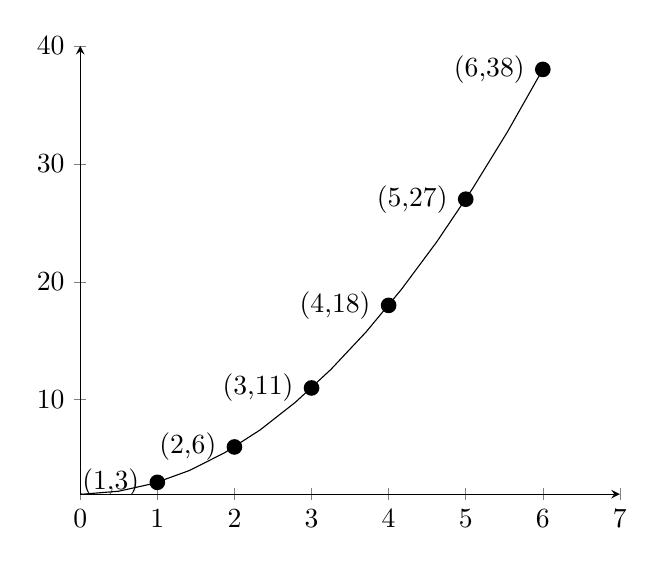
\begin{tikzpicture}
    \begin{axis}[axis y line=middle,axis x line=bottom, xmin=0,xmax=7,ymax=40, domain = -5:6]
        \addplot[mark=none] {x^2+2};
        \node[label={180:{(1,3)}},circle,fill,inner sep=2pt] at (axis cs:1,3) {};
        \node[label={180:{(2,6)}},circle,fill,inner sep=2pt] at (axis cs:2,6) {};
        \node[label={180:{(3,11)}},circle,fill,inner sep=2pt] at (axis cs:3,11) {};
        \node[label={180:{(4,18)}},circle,fill,inner sep=2pt] at (axis cs:4,18) {};
        \node[label={180:{(5,27)}},circle,fill,inner sep=2pt] at (axis cs:5,27) {};
        \node[label={180:{(6,38)}},circle,fill,inner sep=2pt] at (axis cs:6,38) {};
    \end{axis}
\end{tikzpicture}
\end{align*}
\textbf{B24:}\\
\begin{align*}
  A=\{-4,-3,-2,-1,0,1,2\}=\\
  A=\{x \in \mathbb{Z}|-4 \leq x \leq 2\}
\end{align*}
\textbf{C34:}\\
\begin{align*}
  \text{Let } A= |\{x \in \mathbb{N} | |x| < 10\}|\\
  A=\{1,2,3,4,5,6,7,8,9\}\\
  |A|=9
\end{align*}

\section{Section 1.2: B12,B14}
\textbf{B12:}\\
\begin{align*}

\end{align*}
\end{document}
